\documentclass[a4paper,12pt]{article}
\usepackage{amsmath,amsfonts,amsthm,amscd,amssymb,latexsym,comment,eufrak}
%%%%%%%%%%%%%
\usepackage{enumerate,graphicx,psfrag,subfigure}%,jchangebar,oldgerm}
\usepackage[mathscr]{eucal}
\usepackage[usenames]{color}
\usepackage{url}
%\usepackage{showkeys}
%%%%%%%%%
\sloppy
%%%%%%%%%%%%%%%%%%%%%%%
%
%
%
\title{The subgroup membership problem
}
\author{ 
}
%%%%%%%%%%%%%%%%%%%%%%%%%%%
%%%%%%%%%%%%%%%%%%%%%%%%%%%
\renewcommand{\a}{\alpha }
\renewcommand{\b}{\beta }
\newcommand{\G}{\Gamma }
\newcommand{\g}{\gamma }
\newcommand{\D}{\Delta }
\renewcommand{\d}{\delta }
%\def\vd{\vardelta}
\newcommand{\ep}{\epsilon }
\newcommand{\e}{\varepsilon }
\newcommand{\z}{\zeta }
%\eta
\renewcommand{\th}{\theta }
\newcommand{\T}{\Theta }
\renewcommand{\i}{\iota }
\renewcommand{\k}{\kappa }
\renewcommand{\l}{\lambda }
\renewcommand{\L}{\Lambda }
%\mu
%\nu
%\xi
%omicron
%\pi
\renewcommand{\r}{\rho }
\newcommand{\s}{\sigma }
\renewcommand{\S}{\Sigma }
\renewcommand{\t}{\tau }
\newcommand{\up}{\upsilon }
\newcommand{\U}{\Upsilon }
%\phi
\newcommand{\x}{\chi }
%\psi
\newcommand{\W}{\Omega }
\newcommand{\w}{\omega }
%%%%%%%%%%%%%%%%%%%%%%%%%%%%%%%
%%%%%%%%%%%%%%%%%%%%%%%%%%%%%
\def\pd{\partial}
\def\wht{\widehat}
%\def\cC{{\mathcal C}}
%\newcommand{\cdim}{\texttt{cdim}}
\def\fC{{\textswab C}}
%
\def\cD{{\cal{D}}}
\def\cF{{\cal{F}}}
\def\cH{{\cal{H}}}
\def\cJ{{\cal{J}}}

\def\cK{{\cal{K}}}
\def\cP{{\cal{P}}}
\def\cR{{\cal{R}}}
\def\cS{{\cal{S}}}
\def\cW{{\cal{W}}}
\def\cQ{{\cal{Q}}}
%\newcommand{\GG}{\ensuremath{\mathbb{G}}}
\newcommand{\pp}{\mathbf{p}}
%%%%%%%%%%%%%%%%%%%%%%%%%%%%%%
\def\nul{\emptyset }

%%%%%%%%%%%%%%%%%%%%%%%%%%%%%%
\newtheorem{theorem}{Theorem}[section]
\newtheorem{lemma}[theorem]{Lemma}
\newtheorem{corollary}[theorem]{Corollary}
\newtheorem{proposition}[theorem]{Proposition}
\newtheorem{axiom}[theorem]{Axiom}
\newtheorem{definition}[theorem]{Definition}
\newtheorem*{defn*}{Definition}
\newtheorem{conjecture}[theorem]{Conjecture}
%cvs -d :pserver:najd2@cvs.mas.ncl.ac.uk:/CVS/najd2
\newtheorem{exam}[theorem]{Example}
%
%
\newenvironment{example}{\begin{exam} \rm}{\end{exam}}
%
%
%
\newtheorem{remk}[theorem]{Remark}
\newenvironment{remark}{\begin{remk} \rm}{\end{remk}}
%
%%%%%%%%%%%%
\numberwithin{equation}{section}
\numberwithin{figure}{section}
%%%%%%%%%%%%%%%%%%%%
\newcommand{\Iso}{\operatorname{Isom}}
\newcommand{\Aut}{\operatorname{Aut}}
%%%%%%%%%%%%%%%%%%%
\renewcommand{\AA}{\ensuremath{\mathbb{A}}}
\newcommand{\ZZ}{\ensuremath{\mathbb{Z}}}
\newcommand{\QQ}{\ensuremath{\mathbb{Q}}}
\newcommand{\RR}{\ensuremath{\mathbb{R}}}
\newcommand{\NN}{\ensuremath{\mathbb{N}}}
\newcommand{\CC}{\ensuremath{\mathbb{C}}}
\newcommand{\FF}{\ensuremath{\mathbb{F}}}
%\renewcommand{\ker}{\verb"Ker"}
\newcommand{\cC}{\mathcal{C}}
\newcommand{\cO}{\mathcal{O}}
\newcommand{\la}{\langle}
\newcommand{\ra}{\rangle}
%\newcommand{\BA}{\ensuremath{\mathbb{A}}}
%%%%%%%%%%%%%%%%%%%%%%%%%%%%%%%%%%%%%%
\newcommand{\maps}{\rightarrow}
\newcommand{\ov}[1]{\overline{#1}}
\newcommand{\bs}{\backslash}
%%%%%%%%%%%%%%%%%%%%%%%%%%%%%%%
\newcommand{\be}{\begin{enumerate}}
\newcommand{\ee}{\end{enumerate}}
\newcommand{\bd}{\begin{description}}
\newcommand{\ed}{\end{description}}
%%%%%%%%%%%%%%%%%%%%%%%%%%%%%%%%%%% 
%
\newenvironment{ajd}{\noindent\color{blue} AJD }{}
\newenvironment{xxx}{\noindent\color{red}}{}
%
\begin{document}
\maketitle
\section{Double coset normal form}
Based on notes copied (laboriously) from Christian's page 
\url{
http://checkmyworking.com/misc/writemaths/?doublecoset
}

$F_1$, $F_2$ free groups (finitely generated by $X_1$ 
and $X_2$, respectively).

Let $H_1 \leq F_1$, $H_2 \leq F_2$ such that 
there exists an isomorphism $\phi: H_1 \rightarrow H_2$.

i.e. we have finite bases $\{h_1, \ldots, h_m \}$  for $H_1$ and 
$\{h_1', \ldots, h_m'\}$ for $H_2$.

Consider the free group $F(Z)$, generated by $Z=\{z_1, \ldots, z_m\}$, 
and the maps $\phi_1$ and $\phi_2$ such that 
$\phi_1(z_i)=h_i(X_1)  $ and  $\phi_2(z_i)=h^\prime_i(X_2)$, $i=1,\ldots ,m$.
Thus $\phi_i$ extends to an isomorphism of $F(Z)$ to $H_i$. 

Let ${G = F_1 \underset{H_1=H_2}{\ast} F_2}$, the group with  
 presentation $\la X_1,X_2 | h_i = h_i', i=1 \ldots m\ra$.

A  set $S_i \subseteq F_i$ such that
\be 
\item
$F_i = \displaystyle{\bigcup_{s \in S_i} H_isH_i}$ 
and 
\item
for all $s, s^\prime \in S_i$, $s\in H_i s^\prime H_i$ 
implies $s=s^\prime$,
\ee
is called a set of \emph{double coset representatives for} $H_i\le F_i$. 
(We shall assume $S_i$ is infinite.) 

Let $S_1$ and $S_2$ be sets of  double coset representatives of 
$H_1\le F_1$ and $H_2\le F_2$, respectively. Let $g \in G$. 
A word $w$ representing $g$ is in \emph{(double coset) normal form} if 
$w = h_{1}p_1h_{2}p_2 \cdots h_{k}p_kh_{{k+1}}$, with
\be
\item $p_i \in S_1\cup S_2$  and $h_i \in F(Z)$ and
\item if $p_i\in S_j$ then $p_{i+1}\notin S_j$, for $j=1$ and $2$,
\ee
for $i = 1 \ldots k+1$.
\section{Finding double coset representatives}
\begin{comment}
Suppose $g = g_1g_2 \cdots g_k$, where $g_i$ is in a factor $F_1$ or 
$F_2$: that is (after free cancellation if necessary) $g_i$ is a 
reduced word in $(X_1\cup X_1^{-1})^\ast$ or $(X_2\cup X_2^{-1})^\ast$
\end{comment}
Given an arbitrary word $g\in F_1\ast F_2$,  
we should like an algorithm to write $g$ in double coset normal form
with respect to some choice of double coset representatives. We may 
assume (after free cancellation if necessary) that $g$ is a 
reduced word in $((X_1\cup X_2)\cup ( X_1^{-1}\cup X_2^{-1}))^\ast$.
 
First we say $g$ is in \emph{reduced form} if $g = g_1 \cdots g_k$, where
$g_1 \in F_1$ or $g_1 \in F_2$ and 
for 
$k > 1$,    $g_i \in F_i \backslash H_i$, for $i=1$ or $2$ 
 and $g_i$, ${g_{i+1}}$ belong to different factors. As $F_1$ and 
$F_2$ have solvable subgroup membership problem we can rewrite $g$ in
reduced form. More precisely, we construct a Stallings automaton $A_i$ for
$H_i\le F_i$ and choose a maximal subtree $T_i$ of $A_i$. 
Then we write $g=f_1\cdots f_r$, in free product normal
form (each $f_i$ in a factor and successive terms from different factors).
Now using the appropriate Stallings automata we write $f_r=h_rs_r$, where
$h_r\in H_i$ and $s_r$ is a coset representative. (Read the maximal 
possible left prefix $w_r$ of $f_r$ in $A_i$. Then $h_r$ is the 
maximal subword of $w_r$ which belongs to $H_i$ and $s_r$ is the
unique word such that $f_r=h_rs_r$, reduced as written.)

Using the maps $\phi_1$ and $\phi_2$ we now write $h_r$ in terms of the
generators of the other factor, to obtain $h^\prime_r$ and then 
replace $f_{r-1}$ with $f_{r-1}h^\prime_r$. Now begin again with
$f_{r-1}$ instead of $f_r$. Continue till the word is exhausted.   
This gives $g=g_1\cdots g_t$ in reduced form.

To rewrite in double coset normal form we need to  
 rewrite
each $g_i$ in double coset normal form in its factor, 
with respect to some (fixed) set
of double coset representatives.  
We now show how to do this.
\subsection{Double coset representatives}
Let $X$ be a finite alphabet, $F=\FF(X)$ and $H$ a finitely generated subgroup
of $F$.  By a {\em reduced} word we mean (in
this section) a freely reduced word in $(X\cup X^{-1})^\ast$, and we write $w\in F(X)$
to mean that $w$ is a reduced word. For $u,v, w\in F(X)$ we 
write $w=u\circ v$ if $|w|=|u|+|v|$, in which case we say that $u$ is a {\em prefix}
of $w$. 

Let $A$ be the Stallings automaton for $H$. We regard $A$ as a 
labelled directed graph
and refer to its states as {\em vertices}. The label of an edge $e$ is denoted 
$l(e)$ and this notation is extended to paths in the obvious way. 
Fix a spanning tree $T$ for $A$. For 
each vertex $v$ of $A$ let $w(v)$ denote the label of the path from $1$ to $v$ in
$T$. We say the word $w$ is {\em readable} by $A$ if, starting in the 
start state $1$ with input $w$, the automaton finishes with the empty
word in some arbitrary state. If $w$ is readable by $A$ we denote the final
state of $A$ after reading $w$ (starting in state $1$) by $\t(w)$. 
If $w$ is readable by $A$ and $\t(w)=1$
 then we say $w$ is {\em accepted} by $A$. Define 
\[L_T=\{w(v): u \textrm{ is a vertex of } A\}.\]  
If $w, s\in F(X)$ then we say that $s$ is a {\em maximal} $L_T${\em -prefix} of $w$ if 
$s\in L_T$, $w=s\circ v$ and no longer prefix of $w$ belongs to $L_T$. 

We shall define a set of double coset representatives for $H$ in two parts. 
First, a word $w\in F(X)$ is a {\em representative of type} $1$ if 
\[w=s\circ e \circ t^{-1},\]
where $s$ is a maximal $L_T$-prefix of $w$, $t$ is a maximal $L_T$-prefix of 
$t\circ e^{-1}$ and $e\neq 1$. Let $S_1$ denote the set of all representatives of 
type $1$. 

To describe the remaining representatives we shall first define an equivalence
relation on the ordered pairs of distinct vertices of $A$. Let
\[P=\{(u,v)\in V(A)\times V(A): u\neq v\}.\]
Define a relation $\sim$ on $P$ by $(u_0,u_1)\sim (v_0,v_1)$ if and only if 
there exist paths $p_0$ and $p_1$ in $A$, from $u_0$ to $v_0$ and $u_1$ to $v_1$ 
respectively, such that $l(p_0)=l(p_1)$. (We allow these paths to have length $0$.)
It is easy to verify that $\sim$ is an equivalence relation on $P$. 

\begin{lemma}\label{lem:equiv_verts}
Let $(u_0,u_1)$ and $(v_0,v_1)$ be elements of $P$ and let 
$a_0=w(u_0)$, $a_1=w(u_1)$, $b_0=w(v_0)$ and $b_1=w(v_1)$. Then 
$(u_0,u_1)\sim (v_0,v_1)$ if and only if there exist $h_0,h_1\in H$ such that
\[a_0a_1^{-1}=h_0b_0b_1^{-1}h_1^{-1}.\]
\end{lemma}  
\begin{proof}
$\Rightarrow$: Let $p_0$ and $p_1$ be paths, from $u_0$ to $v_0$ and $u_1$ to $v_1$ 
respectively, such that $l(p_0)=l(p_1)=c$, say. Set $h_0=a_0cb_0^{-1}$ and 
$h_1=a_1cb_1^{-1}$. Since $h_0$ and $h_1$ are labels of closed paths based at $1$ we
have $h_0$ and $h_1$ in $H$. Thus 
$a_0a_1^{-1}=h_0b_0c^{-1}cb_1^{-1}h_1^{-1}=h_0b_0b_1^{-1}h_1^{-1}$, as required.

$\Leftarrow$: Let $h_0$, $h_1 \in H$ such that $a_0a_1^{-1}=h_0b_0b_1^{-1}h_1^{-1}$. 
Set $k=a_0^{-1}h_0b_0=a_1^{-1}h_1b_1$. Then $h_0=a_0kb_0^{-1}$ and $h_1=a_1kb_1^{-1}$
belong to $H$ so there exist paths $p_0$ and $p_1$, 
from $\t(a_0)=u_0$ to $\t(b_0)=v_0$ and 
$\t(a_1)=u_1$ to $\t(b_1)=v_1$, both with labels $k$. 
Therefore $(u_0,u_1)\sim (v_0,v_1)$. 
\end{proof}  

We shall choose one double coset representative corresponding to each $\sim$ 
equivalence class. To be explicit we make a particular choice of transversal
for the equivalence classes, as follows. 
If $(u,v)\in P$ and $w(u)=a\circ x$, $w(v)=b\circ x$, for some $a,b\in F(X)$ and 
$x\in X^{\pm 1}$, then $(\t(a),\t(b))\in P$ and $(u,v)\sim (\t(a),\t(b))$. It follows
that every equivalence class of $\sim$ contains an element $(a,b)$ such that
$w(a)w(b)^{-1}$ is a reduced word. Let $\pp$ be an equivalence class of $\sim$ and
let $Y$ be the set of all pairs $(u,v)\in \pp$ such that $|w(v)|$ is minimal (amongst
elements of $\pp$). Choose $(u,v)\in Y$ such that $|w(u)|$ is minimal (amongst elements
of $Y$) and define $(u,v)$ to be the $\sim${\em representative} of $\pp$. Fix
one $\sim$ representative for each equivalence class of $\sim$ and  
let $Q$ denote the set of  all these $\sim$ representatives. A word $w\in F(X)$ is
 a {\em representative of type} $2$ if $w=w(u)w(v)^{-1}$, for some $(u,v)\in Q$. 
Let $S_2$ denote the set of all representatives of type $2$ and define $S=S_1\cup S_2$.
(Note that by the minimality conditions of the defintion, if $(u,v)$ is a 
$\sim$ representative then $w(u)w(v)^{-1}=w(u)\circ w(v)^{-1}$.)

\begin{proposition}\label{prop:dcreps}
$S$ is a set of double coset representatives for $H$.
\end{proposition}   
\begin{proof}
First we shall show that every element $w\in F(X)$ lies in $HdH$, for some $d\in S$. 
In fact we describe an algorithm which rewrites a given word $w$ in this form. 

Assume that the Stallings automaton $A$ for $H$ has been constructed by folding from
given generators for $H$. A spanning tree for $A$ may then be found and the 
set $L_T$ computed. For each pair $(u,v)\in P$ the equivalence class $\pp$ of 
$(u,v)$ may be constructed by considering all simple paths (no repeated vertices)
from $u$ to $v$. A pair $(u^\prime ,v^\prime) \in P$ belongs to $\pp$ if and only
if $u^\prime$ lies on a simple path beginning at $u$ and $v^\prime$ lies on 
a simple path beginning at $v$. Having constructed the equivalence classes of $\sim$
 a set of $\sim$ representatives may be constructed, by considering the 
lengths of $w(a)$ and $w(b)$ for all $(a,b)$ in an equivalence class. Thus the
sets $Q$ and $S_2$ may be computed.   \\

\noindent{\bf The algorithm}:\\
Input $w\in F(X)$. 
Let $h$ be the maximal prefix of $w$ accepted by $A$; so $h\in H$ and 
$w=h\circ f$, for some $f\in F(X)$. Now use $A$ to find the maximal $L_T$-prefix $p$ 
of $f$ (that is the maximal prefix which is readable by $A$)
 so $f= p\circ q$, for some $q\in F(X)$. 

Next find the maximal prefix $g$ of $q^{-1}$ acceptable by $A$: say 
$q^{-1}=g\circ r$, for some $r\in F(X)$, and then the maximal $L_T$-prefix 
$t$ of $r$ which
is readable by $A$; say $r=t\circ e^{-1}$, for some $e\in F(X)$. 

If $e\neq 1$ then
\[w=h\circ p \circ e\circ t^{-1}\circ g^{-1},\]
with $h,g\in H$. In this case $p$ and $t$ are readable by $A$. Set $y=w(\t(p))$
and $z=w(\t(t))$. Then $py^{-1}$ and $tz^{-1}$ belong to $H$. Moreover, as $p$
is a maximal $L_T$-prefix of $f$ it is also a maximal $L_T$-prefix of $pet^{-1}$ and so
  the 
first letter of $e$ is not readable from the vertex $\t(p)=\t(y)$. In particular
$ye=y\circ e$. Similarly, the first letter of $e^{-1}$ is not readable from
the vertex $\t(t)=\t(z)$, so $ez^{-1}=e\circ z^{-1}$. Moreover $y$ is a 
maximal $L_T$-prefix of $yez^{-1}$ and $z$ is a maximal $L_T$-prefix of $ze^{-1}$. 
Thus $yez^{-1}\in S_1$ and we output
\[w=(py^{-1}) (yez^{-1})(zt^{-1})\in HSH,\]
of the required form.

On the other hand if $e=1$ then 
\[w=h\circ p\circ t^{-1}\circ g.\]
In this case let $u=\t(p)$ and $v=\t(t)$ and let $(u_0,v_0)$ be the $\sim$ representative
of the equivalence class of $(u,v)$.  Let $y=w(u_0)$ and $z=w(v_0)$. Then,  from Lemma
\ref{lem:equiv_verts}, there exist $h_0,h_1\in H$ such that 
\[w(u)w(v)^{-1}=h_0yz^{-1}h_1^{-1}\]
and we have $p w(u)^{-1}$, $t w(v)^{-1}$ in $H$. Hence 
\[
p\circ t^{-1}=( p w(u)^{-1})w(u)w(v)^{-1}( w(v)t^{-1})=( p w(u)^{-1}) h_0 yz^{-1}
h_1^{-1}( w(v)t^{-1})
\]
and by definition $yz^{-1}\in S_2$. We then output 
\[w=a yz^{-1} b,\]
where $a=h ( p w(u)^{-1}) h_0\in H$ and $b=h_1^{-1}( w(v)t^{-1})g \in H$.

It remains to show that if $s_0,s_1\in S$ with $s_1\in Hs_0H$ then $s_1=s_0$.
Suppose that $s_1=as_0b$, where $a, b\in H$.  
If $s_0\in S_1$, say $s_0=y_0e_0z_0^{-1}$, then, as $ay_0$ and $b^{-1}z_0$ are readable
by $A$ and $e_0\neq 1$, it follows (as above) that $s_1$  
cannot be factored as $s_1=yz^{-1}$,
where both $y$ and $z$ are readable by $A$. Hence both $s_0$ and $s_1$ belong to
$S_1$ or both belong to $S_2$. 

Consider the case where both belong to $S_1$ and, in the usual notation,
$s_i=y_i e_i z_i^{-1}$, $i=0,1$. We have $s_1=as_0b$, $a,b\in H$, and as $y_0$ has
no left divisor in $H$, if $a\neq 1$ then $a$ does not cancel completely with
 a prefix of $y_0$. Thus, if $a\neq 1$ then we may write $a=a_0\circ a_1$ and 
$y_0=a_1^{-1}\circ y_0^\prime$, where $ay_0=a_0\circ y_0^\prime$. Since 
$a$ is accepted by $A$ we have $\t(ay_0)=\t(a_0y_0^\prime)=\t(y_0)$. By definition
of $s_0$ the first letter of $e_0$ is not readable from the vertex $\t(y_0)$, so
it follows, as before that $a_0y_0^\prime e=a_0\circ y_0^\prime \circ e$. Similarly,
if $b\neq 1$ then $b=b_0\circ b_1$ and $z_0=b_0\circ z_0^\prime$, with
$z_0^{-1}b= (z_0^\prime)^{-1}\circ b_1$ and $e (z_0^\prime)^{-1}b_1=
e\circ  (z_0^\prime)^{-1}\circ b_1$. This implies that 
$s_1=a_0\circ y_0^\prime \circ  e\circ  (z_0^\prime)^{-1}\circ b_1$ and by considering 
maximal $L_T$-prefixes of both sides we see that $y_1=a_0\circ y_0^\prime$ and 
$z_1=b_1^{-1}\circ z_0^\prime$. We now have  $\t(y_1)=\t(a_0y_0^\prime)=\t(y_0)$ which
 means that 
$y_0=y_1$ and this in turn implies that $a=1$. Similarly $z_0=z_1$ so $b=1$. 
Hence $s_0=s_1$ in this case.

Finally consider the case where $s_1$ and $s_2$ belong to $S_2$. As $s_1=as_0b$, with
$a,b\in H$, Lemma \ref{lem:equiv_verts} and the definition of $S_2$ imply  that 
$s_0= s_1$. Therefore $S$ is a set of double coset representatives.
\end{proof}



In fact if we don't require uniqueness of representatives then the algorithm 
may be made much simpler than the description above: it can 
simply find the maximal prefix $h_1$ of $w$  accepted  by $A$  and so $w=h_1\circ v$. Then find the
maximal prefix $p$ of $\bar v$ accepted by $A$. Setting $h_2=\bar p$ gives $w=h_1\circ d \circ h_2$, for
some uniquely determined word $d$, which is the (non-unique) 
double coset representative. 


\begin{example}
Picture required: and further work required for the full algorithm.
\begin{align*} 
g &= x_1^3x_2^2y_1y_2 \\ 
&= (x_1^2)(x_1x_2)(x_2^{-1})^{-1} \cdot (y_1)(y_2^{-1})^{-1}
\end{align*}
\end{example}

\subsection{Construction of the normal form}

Now we write each syllable $g_i$ of $g=g_1\cdots g_t$ in normal form using the algorithm above. 
This gives $g_i=h_{i,1}d_ih_{i,2}$, with $d_i\in S_1\cup S_2$. Using $\phi_1$ or $\phi_2$, as appropriate,
we now write $h_{i,1}$ and $h_{i,2}$ as words in $F(Z)$. For $i=1,\ldots , t-1$, we reduce the 
word $h_{i,2}h_{(i+1),1}\in F(Z)$ to give a reduced word $h_i\in F(Z)$ and set $h_0=h_{1,1}$ and  $h_{t+1}=h_{t,2}$.
Then $g$ has normal form $h_0d_1h_1\cdots d_th_{t+1}$.
%
%%%
%
%%%%%%%%%%%%%%%%%%%%%%%%%%%%%%%%%%%%%%%%%%%%%%%%% 
\section{The generalised folding process}
The object is to construct an automaton which will accept a word $w$
in double-coset normal form if and only if it belongs to the subgroup $K$.
The idea is to this by starting with the flower automaton for the 
generators of $K$, written in (double-coset) normal form, carrying out
Stallings folding as usual to produce a deterministic, trim, inversive 
automaton, and next adding some additional paths to allow normal forms
to be read. This may introduce new non-determinism in some  states (i.e.
things not folded), so
the resulting automaton must be folded. We carry on this process as long
as we can: but of course need to show that it halts. Suppose $L$ is the 
language accepted by the flower automaton of $K$. The image of $L$ under
the canonical map to $G$ is $K$. All the stages of our generalised folding
process will preserve this image, so our final automaton will accept a language
$L_1$ which also maps to $K$. We must then prove that if $w$ is a word
in normal form which represents an element of $K$ then $w$ is in $L_1$. It will
therefore suffice to show that if $u$ is any word in $L_1$ then the 
normal form of $u$ is also in $L_1$. 

If things get unpleasant then we  shall restrict to malnormal $H_i$ to make the generalised folding process simpler, but for now we make no such assumption.
 Recall from above that we have 
$F_1$, $F_2$ free groups (finitely generated by $X_1$ 
and $X_2$, respectively); 
 $H_1 \leq F_1$, $H_2 \leq F_2$ such that 
there exists an isomorphism $\phi: H_1 \rightarrow H_2$; a free group 
 $F(Z)$, generated by $Z=\{z_1, \ldots, z_m\}$, 
and  maps $\phi_1$ and $\phi_2$ such that 
$\phi_1(z_i)=h_i(X_1)  $ and  $\phi_2(z_i)=h^\prime_i(X_2)$, $i=1,\ldots ,m$,
both of which induce isomorphisms. 
Implicit in all this is that $X_1\cap X_2=X_1\cap Z = X_2\cap Z=\nul$. 
We define 
${G = F_1 \underset{H_1=H_2}{\ast} F_2}$, the group with  
 presentation $\la X_1,X_2 | h_i = h_i', i=1 \ldots m\ra$ and 
let $S_1$ and $S_2$ be sets of  double coset representatives of 
$H_1\le F_1$ and $H_2\le F_2$, respectively, (as in  the 
previous section).

Let $K=\la k_1, \ldots , k_s\ra$, where $k_i$ is an element of $G$ written
in normal form: say
\begin{equation}\label{eq:k-form}
k_i= h_{i,0}t_{i,1}h_{i,1}\cdots t_{i,m_i}h_{i,m_i+1},
\end{equation}
where $h_{i,j}\in F(Z)$ and $t_{i,j}\in S_1\cup S_2$.   
\subsection{Double-coset automata and graphs}
{\bf We should include a short description of Stallings folding, as in
Enric's notes from Manresa \cite{ventura11}.} \\[1em]

An {\em automaton} $A$ is  a quintuple $(\S,A,\d,S,F)$, 
where $\S$  is finite set called the {\em alphabet}, $Q$ is a finite 
set of {\em states}, $\d$ is a map $\d:Q\times \S\maps Q$, called 
the {\em transition function}, $S\subset Q$ is the (non-empty) 
set of {\em start states} 
and 
$F\subseteq Q$ is the set of {\em final states}. (Usually $S$ is 
a singleton.) If $F=\{s_0\}=S$ it's common
to drop $F$ from the description and define $A$ as a quadruple.
The language accepted by an automaton $A$ (with any choice of start state
in $S$) is denoted $L(A)$. If $G$
is a group generated by $\S$ then the  natural map from $L(A)$ to
$G$ is denoted $\pi:L(A)\maps G$.

We shall associate to an automaton $A$ a directed, edge labelled graph
$\G_A$ with vertices $V=V(\G_A)=Q$,  
edge set $E=E(\G_A)$ consisting
of elements $(u,\s,v)$ of $Q\times \S\times Q$ such that $\d(u,\s)=v$ and 
labelling function $l:E\maps \S$ given by $l(u,\s,v)=\s$, for all $(u,\s,v)
\in E$.  If $A$ has a property (like trim, involutive or deterministic) then
we ascribe this property to $\G_A$ as well. (Although we usually use the term
``folded'' instead of ``deterministic'', for graphs.) If $S$ and $F$ are
the start and final states of $A$ we sometimes write $(\G_A, S,F)$, and
in particular if $S=\{s_0\}$ and $F=\{f_0\}$, we write $(\G_A,s_0,f_0)$ and 
if $S=\{s_0\}$ we  
call $s_0$ the {\em root} vertex of $\G_A$. 

A colouring of a directed, inversive, labelled graph $\G$ is a map $c$  from $V(\G)\cup E(\G)$
 to a set $C$ such that if $\i_E$ is the involution on edges 
then $c(e)=c(\i(e))$. (We make no conditions on the colouring of vertices:
in particular adjacent vertices may have the same colour.)

\begin{definition}
A finite, rooted, directed, labelled, coloured graph $\G$ is called a 
{\em double-coset-graph} or 
{\em dc-graph}
if $\G$ has vertices, edges, labelling function and colouring function,
 $V$, $E$, $l$ and $c$, 
respectively, satisfying the following conditions.
\be[(i)]
\item $l$ is a map $l:E\maps X_1\cup X_2\cup Z$.
\item $c$ is a map $c:V\cup E\maps \ZZ\times \ZZ$. 
\item $E=E_Z\cup E_{X_1}\cup E_{X_2}$,
where $E_Z=l^{-1}(Z)$, $E_{X_1}=l^{-1}(X_1)$ and $E_{X_2}=l^{-1}(X_2)$.
\item $V=V_0\cup V_C$, where $V_C=V\bs V_0$ and 
$V_0$ is the union of 
$V_{X_1}$, $V_{X_2}$ and $V_Z$, with   
$V_Y=\{\textrm{vertices incident only to edges of } E_Y\}$, for $Y=Z,X_1$ or $X_2$. 
\item Let $c_k:V\cup E\maps \ZZ$ be the composition of $c$ with projection
onto the $k$th factor of $\ZZ\times \ZZ$, for $k=1$ or $2$. Then 
$c_k(x)\ge 0$, for all $x\in V\cup E$ and  for $k=1$ and $2$. 
\item Fix $k\in \{1,2\}$.  For all $v\in V$,  
$c_k(v)>0$ if and only if $v\in V_0$. Moreover, if $v\in V_0$ then
$c_k(v)=\max\{c_k(e): e \textrm{ is incident to } v\}$. 
\ee
An automaton $A$ is called a {\em dc-automaton} if $\G_A$ is  a dc-graph.
\end{definition}

\begin{example}\label{ex:dc-graph}
Figure \ref{fig:dc-grapha} shows a dc-graph, with root $\a$, 
where $x\in X_1$, $y_1,y_2,y_3\in X_2$,
$z\in Z$, the only vertex not in $V_0$ is $\d$, 
colours of all edges are shown and the colours of vertices  are 
$c(\a)=(3,0)$, $c(\b)=(3,0)$, $c(\g)=(0,2)$, $c(\d)=(0,0)$, $c(\e)=(0,2)$ and 
$c(\z)=(1,0)$.  
\end{example}
\begin{figure}
\begin{center}
\psfrag{a}{$\a$}
\psfrag{b}{$\b$}
\psfrag{c}{$\g$}
\psfrag{d}{$\d$}
\psfrag{e}{$\e$}
\psfrag{f}{$\z$}
\psfrag{g}{$\eta$}
\psfrag{h}{$\theta$}
\psfrag{x}{$x$}
\psfrag{z}{$z$}
\psfrag{y1}{$y_1$}
\psfrag{y2}{$y_2$}
\psfrag{y3}{$y_3$}
\psfrag{(1,0)}{$(1,0)$}
\psfrag{(0,0)}{$(0,0)$}
\psfrag{(0,2)}{$(0,2)$}
\psfrag{(3,0)}{$(3,0)$}
\subfigure[A dc-graph...]{
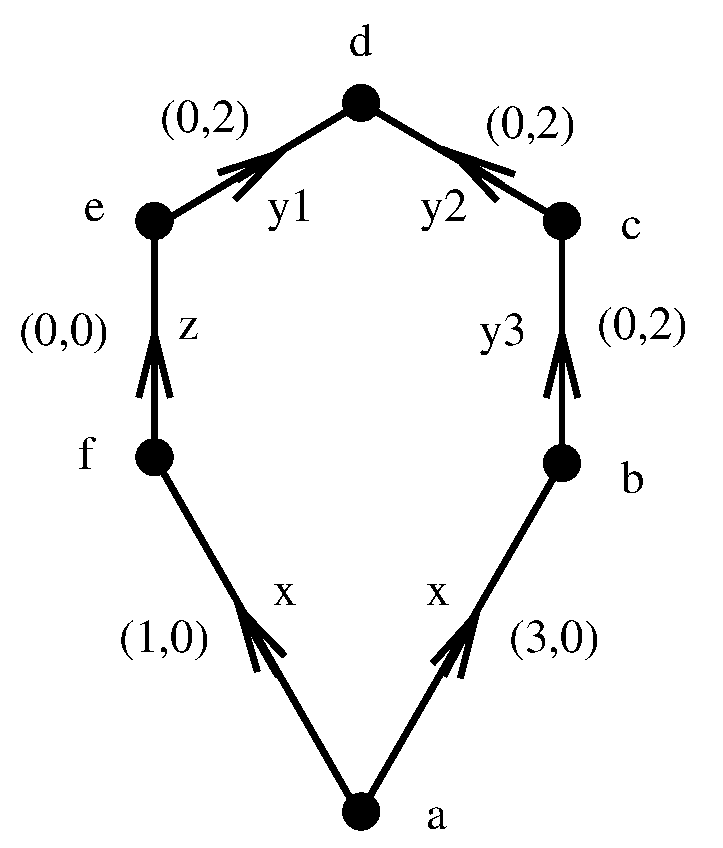
\includegraphics[scale=.5]{dc-graph.eps}
\label{fig:dc-grapha}
}
\hspace{15mm}
\subfigure[... and its Stallings folding]{
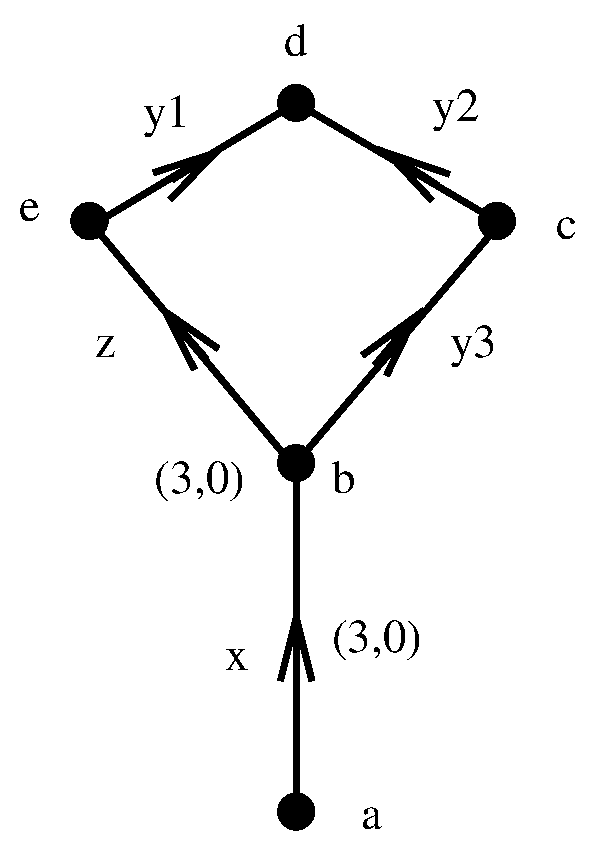
\includegraphics[scale=.5]{dc-folded.eps}
\label{fig:dc-graphb}
}
\end{center}
\caption{Folding a  dc-graph}\label{fig:dc-graph}
\end{figure}
An {\em elementary dc-folding} of a dc-graph $\G$ is a graph $\G^\prime$
obtained from $\G$ as follows. Suppose that $e=(p,a,q)$ and 
$e^\prime=(p,a,q^\prime)$
are edges of $\G$. (We do not require $p$, $q$ and $q^\prime$ to be distinct.) 
% with $c(p)=(m_1,n_1)$, $c(q)=(m_2,n_2)$, 
%$c(q^\prime)=(m_3,n_3)$, $c(e)=(r_1,s_1)$ and $c(e^\prime)=(r_2,s_2)$.
 Then $\G^\prime$ is the quotient of $\G$ formed by identifying 
$q$ and $q^\prime$, to form a new vertex $q^{\prime\prime}$; and 
$e$ and $e^\prime$, to form a new edge 
$e^{\prime\prime}=(p,a,q^{\prime\prime})$. If the root of $\G$ is $q$
 or $q^\prime$ then $q^{\prime\prime}$ is the root of $\G^\prime$ and otherwise
 the root of $\G^\prime$ is that of $\G$. The colouring map of $\G^\prime$
is the same as that of $\G$ except that  
 $c_k(\e^{\prime\prime})=\max\{c_k(e),c_k(e^{\prime\prime})\}$ 
and $c_k(q^{\prime\prime})=\max\{c_k(q),c_k(q^{\prime\prime})\}$,
for $k=1,2$. 
From the definition, the conditions for a dc-graph are satisfied by 
$\G^\prime$. A {\em dc-folding} of a dc-graph $\G$ is a graph obtained 
from $\G$ by a finite sequence of elementary foldings. Thus a dc-folding 
of a dc-graph is again a dc-graph. 

From now on we shall assume, unless we explicitly indicate otherwise,
 that all graphs are dc-graphs and  all foldings are dc-foldings. 
A graph on which  it is not possible to perform an elementary
folding is 
said to be {\em folded}. A {\em Stallings folding} of a graph $\G$ is
 a (possibly trivial) folding of $\G$ which is folded. As every non-trivial 
folding dedreases
 the number of edges of the graph, every graph has a Stallings folding. From the
standard theory (e.g. Enric's notes \cite{ventura11}) a Stallings folding of a graph is unique,
so we may define {\em the Stallings folding} $S(\G)$ of a graph $\G$.\\
({\bf This is not quite clear, because it needs to be established that colouring
of a Stallings folding of $\G$ is not dependent on  the order of folding. It 
would be enough to show that the morphism from $\G$ to $S(\G)$ is uniquely 
determined by $\G$, but I haven't checked this out.})
\begin{example}
Figure \ref{fig:dc-graphb} shows the Stallings folding of the graph of 
Example \ref{ex:dc-graph}. Colours are shown only where the folding changes them.
\end{example}
%
%
Now let $\cF(K)$ be the flower automaton of $K$ and let 
$\G$ be the corresponding rooted graph. If $e$ is an edge of $\G$ then
$e$ is labelled by a letter (of $X_1\cup X_2 \cup Z$) 
occuring in $h_{i,j}$ or $t_{i,j}$, for some $i,j$, as in 
\eqref{eq:k-form}. If $e$ is labelled by a letter of $Z$ we say $e$ has {\em type} $Z$
and define $c(e)=(0,0)$. If $e$ is labelled by a letter of $X_k$ occuring in 
$t_{i,j}$, we say $e$ has {\em type} $X_k$ and define 
\[c_k(e)=m_1+\cdots m_{i-1} +j\textrm{ and } c_{k^\prime}(e)=0,\]
where $k\neq k^\prime$. If $v\in V_C$ then we define $c(v)=(0,0)$. If $v\in V_0$ then
 we define $c_k(v)=\max\{c_k(e): e \textrm{ is incident to } v\}$, for $k=1,2$.  
This makes $\G$ into a dc-graph. The graph of Example \ref{ex:dc-graph} is obtained 
from the subgroup $K$ generated by the single element $xzy_1y_2y_3x^{-1}$ in this way.

Now let $\D$ be the Stallings folding of the dc-graph $\G$.  Then
 $\D$ is a connected, deterministic, trim, dc-graph and $\pi(L(\D))=K$. However
$L(\D)$ does not, in general, contain all normal forms of elements of $K$. 
Next we enlarge $\D$ to allow it to accept normal forms. 
\begin{definition}\label{def:attractive}
Let $\D$ be a  dc-graph, let $k\in \{1,2\}$ and let 
$u,v\in V_0(\D)$ such that 
\be[(i)]
\item $c_k(u)\neq c_k(v)$ and 
\item there exists a path $p$ from $u$ to $v$ in $\D$ with label $l(p)$ 
a word in $F(X_k\cup Z)$. 
\ee
Then the pair $(u,v)$ is said to be 
$k${\em -attracting} with {\em link} $p$ and {\em resolution} 
$r(u,v)$ the normal
form of $l(p)$ in $F(X_k)$. 
\end{definition}

We set 
\begin{align}
A_k&=\{\{u,v\}\subseteq V_0(\D): (u,v) \textrm{ is an attracting pair}\} \textrm{ and }\\\label{eq:attset}
\vec{A_k}&=\{(u,v)\in V_0\times V_0: \{u,v\}\in A_k\}.
\end{align}
As a direct consequence of the definitions we have the following lemma.
\begin{lemma}
If $\{u,v\}$ and $\{v,w\}\in A_k$ and $c_k(u)\neq c_k(v)$ then 
$\{u,w\}\in A_k$.
\end{lemma}
Let $\D_k$ be the graph formed from $\D$ by removing all edges of type
$X_{k^\prime}$, where $k\neq k^\prime$. An $X_k$ component of $\D_k$ is 
the subgraph of $\D$ formed from a connected component of $\D_k$ by removing
all leaves which are incident to edges of type $Z$, and then repeating the
process till there are no such leaves left. 
 We shall modify the $X_k$ components of $\D_k$ so that normal forms of words 
are readable. 

Let $\T$ be an $X_k$ component of $\D_k$. If $(\a,z,\b)$ is an edge of 
$\T$ labelled by an element $z\in Z$ then add a path from $\a$ to 
$\b$ labelled by $\phi_1(z)$ to the graph $\T$. Do this for all such edges
and call the result $\T_1$.   A 
{\em boundary vertex} of $\T_1$ is defined to be a vertex
$\a$ such that $\a$ is incident, in $\D$, to a vertex which does not
belong to $\T_1$.  

Given labelled 
graphs $\G_1$ and $\G_2$ we define the {\em product} graph $G_1\times G_2$
to be the graph with vertices $V=V(G_1)\times V(G_2)$ and with a directed
edge labelled $a$ from $(u_1,u_2)$ to $(v_1,v_2)$ if and only if there are 
edges $(u_1,a, v_1)$ and $(u_2,a,v_2)$ in $\G_1$ and $\G_2$, respectively. 
Let $P=\T_1\times \G_{A_k}$. Then there is a path labelled $w$ from 
$\a$ to $\b$ in $T_1$ and a path labelled $w$ from $\a^\prime $ to $\b^\prime$
in $\G_{A_k}$ if and only if there is a path labelled $w$ from $(\a,\a^\prime)$ to
$(\b,\b^\prime)$ in $P$. Choose a spanning  subtree $\U$ of  $P$. We shall
use $P$ to add new paths to $\T_1$. First order the vertices of
$\T_1$: say these are $\a_0,\ldots, \a_t$, in the given order.

Let $\a_i$, $\a_j$ be vertices of  $\T_1$ with $i\le j$. If  
there exists a simple path $p$ in $P$ from $(\a_i,1)$ to $(\a_j,1)$ then let 
$l_p\in F(X_k)$ be the label of $p$ and let $w_p=\phi_k^{-1}(l_p)\in F(Z)$. 
Let $q$ be a path (disjoint from $\T_1$) of length $|w_p|$ and with 
label $w_p$. Identify the intial vertex of $q$ with $\a_i$ and the 
terminal vertex of $q$ with $\a_j$. Now fold the resulting graph. Repeat
this process for all simple paths from  $(\a_i,1)$ to $(\a_j,1)$, over
all pairs of vertices $\a_i$, $\a_j$ with $i\le j$. Call the resulting
graph $\T_2$. There are finitely many simple paths in $P$ so this process
terminates. Moreover, regarding $\T_1$ and $\T_2$ as automata, if $\a$ and
 $\b$ are
boundary vertices of $\T_1$ and $L_1$ and $L_2$ are the
languages accepted by $(\T_1,(X_k\cup Z), \a,\b)$ and 
$(\T_2,(X_k\cup Z), \a,\b)$, respectively, then $\pi(L_1)=\pi(L_2)\subseteq G$.

As the edges added to $\T_1$ to form $\T_2$ are all labelled by elements 
of $Z$, and all edges of $\G_{A_k}$ are labelled by elements of $X_k$ 
the graphs $P=\T_1\times \G_{A_k}$ and $\T_2\times \G_{A_k}$ differ only
in that the second may have some new isolated vertices. For our purposes
we may discard these and assume that $P=\T_1\times \G_{A_k}=
 \T_2\times \G_{A_k}$. If $P=\U$ then we have nothing to do at the
next stage and we immediately set $\T_3=\T_2$. Otherwise, 
suppose that $e$ is an edge of $P$ which does not belong to $\U$ but
which does belong to a component $\Xi$  of $P$ containing a vertex
$(\a,1)$, for some vertex $\a$ of $\T_2$. 
Let $(\a,1)$ be such a vertex and let 
$e=((\a_i,\b_1), x, (\a_j,\b_2))$, 
with $i\le j$ and with label $x\in X_k^{\pm 1}$. 
%Let 
%$\a_m$ be the minimal vertex of $\T_2$ (necessarily also a vertex
%of $\T_1$)  such that $(\a_m,1)$ belongs to $\Xi$.    
 Let $p_i$ be   
the path in $\U$ from $(\a,1)$ to $(\a_i,\b_1)$ and let $p_j$ be
the path in $\U$ from  $(\a_j,\b_2)$ to $(\a,1)$ and 
let $l_i$ and $l_j$ be the labels of $p_i$ and $p_j$, respectively. Then 
$p_i,e,p_j$ projects to a closed path in $\G_{A_k}$, based at $1$, with
label $h_e=l_i x l_j \in H_k\subseteq F_k$. Moreover   
$p_i,e,p_j$ projects to a closed path in $\T_2$, based at $\a$, also 
with label $h_e$. Let 
$w_e=\phi_k^{-1}(h_e)$ and let 
$q$ be a path (disjoint from $\T_2$) of length
$|w_e|$ and with label $w_e$. Identify the initial and terminal 
vertices of $q$ to $\a_i$ and $\a_j$, respectively, and fold the
resulting graph. Repeat this process for all such edges $e$ and 
vertices $(\a,1)$ of $P$
and denote the result by $\T_3$. If 
$L_3$ is the
language accepted by $(\T_3,(X_k\cup Z), \a,\b)$, for boundary
vertices $\a$, $\b$ of $\T_3$, then again $\pi(L_3)=\pi(L_1)$. 
Later we shall show that if a word $w$ belongs to $H_k\subseteq F_k$ and 
$L_1$ then
$\phi_k(w)$ belongs to $L_3$. (In practice it's not necessary to 
repeat this process for {\em all} such vertices $(\a,1)$ in $\Xi$: but it
makes the proofs later easier if we assume that we do so.)

Next we wish to add paths to $\T_3$ that allow us to read the normal
form of words $w$ which are readable by $\T_3$ and readable 
(but not accepted) by $\G_{A_k}$.  
As before we may assume that
$P=\T_1\times \G_{A_k}=
 \T_3\times \G_{A_k}$. 
Recall that we have fixed a spanning subtree 
$T_k$ of $\G_{A_k}$. Let $p$ be a simple path in $P$ from a 
vertex $(\a_0,1)$ to a vertex $(\a_1,\b_1)$, containing no
vertices of the form $(\a,1)$ except the first. If $P$ contains a 
path from $(\a_0,1)$ to $(\a_1,\b_1)$ which projects onto $T_k$ then
 say that $P$ {\em covers} $p$. 
If all such paths are covered by $P$ then set $\T_4=\T_3$.
Otherwise 
let $p$ be a simple path in $P$ from a  vertex $(\a_i,1)$ to a vertex $(\a_j,\b)$, containing no further
vertices of the form $(\a,1)$,
which is not covered by $P$.
 Let 
$p$ have label $a$.  
Let $b$ be label of the path in $T_k$ from $1$ to $\b$. 
Then $ab^{-1}=h\in H_k\in F_k$. Let 
$w=\phi_{k}^{-1}(ab^{-1})
\in F(Z)$ and let $q$ be a path with label $wb$. Identify the initial
and terminal vertices of $q$ with vertices $a_i$ and $a_j$ of $\T_3$, 
respectively, and fold
the resulting graph. 
As $\pi(a)=\pi(wb)\in G$ the image of the language accepted by
the resulting graph (considered as an automaton) is unchanged by
this operation. 
Repeat this process for all such paths $p$ in $P$ and 
call the result $\T_4$. 

Finally we wish to add paths which allow double-coset representatives
of type $2$ to be read. Suppose $(\e,\xi)\in \G_{A_k}\times \G_{A_k}$ and
that the $\sim$ representative of $(\e,\xi)$ is $(\e_0,\xi_0)$. If there
exist paths $p_1$ from $(\a_i,1)$ to $(\a_j,\e)$ and $p_2$ from
$(\a_l,1)$ to $(\a_j,\xi)$, in $P$,  then let $b_1$ and $b_2$ be the labels
of paths $w(\e)$ and $w(\xi)$, from $1$ to $\e$ and $1$ to $\xi$ in the
subtree $T_k$ of $\G_{A_k}$. Let $a_1$ and $a_2$ be the labels of 
paths $w(\e_0)$ and $w(\xi_0)$. Then there is a path with label 
$c$ from $\e$ to $\e_0$ and from $\xi$ to $\xi_0$. Let $h_i=
b_ica_i^{-1}\in H_k$ and let $w_i=\phi_k(h_i)$, for $i=1,2$. 
Let $q$ be a path with label $w_1 a_1a_2^{-1} w_2^{-1}$ 
and identify the initial
and terminal vertices of $q$ to  vertices $\a_i$ and $\a_l$
of $\T_4$, respectively. 
Fold the resulting graph. 
To see that the image of the language accepted by
 the new graph is the same as that of the original note
that the word $b_1b_2^{-1}$ is readable, starting at $\a_j$ and 
ending at $\a_l$, in $\T_4$. As $\pi(b_1b_2{-1}=\pi(w_1a_1a_2^{-1}w_2^{-1})$
the addition of this new path has no effect on the image of the language 
under $\pi$.  
%$d_1$ and
%$d_2$ be labels of paths $p_1$ and $p_2$ in $P$ and let $e_1$ and 
%$e_2$ be labels of simple paths with the same end points. Then 
%$d_ie_i^{-1}\in H_k$ and  there is a path
%in $\T_4$ with label $\phi_k(d_ie_i^{-1})e_i$, for $i=1,2$. Moreover,
%$\T_4$ contains a path
%with label $\phi_k(e_ib_i^{-1})b_i$ and so a path with label
%$\phi(d_ib_i^{-1})b_i$, $i=1,2$.  
Repeat this process for all such 
pairs $(\e,\xi)$ to form $\T_5$.    

\begin{lemma}
Let $\a$ and $\b$ be boundary vertices of $\T_1$ and let $w$ be a word
 which is accepted by the automaton $(\T_1, X_k\cup Z, \a, \b)$. Then the
normal form of $w$ is accepted by $(\T_5, X_k\cup Z, \a, \b)$. 
\end{lemma}
\begin{proof}
There are two cases to consider, depending on the nature of the 
normal form of $w$. First 
let $w$ have normal form $h_1 a_1 c a_2^{-1} h_2^{-1} $, where 
$h_1$ and $h_2$ are in $F(Z)$,  $a_1$ and $a_2$ are labels 
of simple paths in the subtree $T_k$ and $c$ and $c^{-1}$ have
no non-trivial prefix readable in $A_k$. Then there are words
$g_1, g_2, b_1$ and $b_2\in F(X_k)$ such that 
$w=g_1\circ b_1\circ c \circ b_2^{-1}\circ g_2^{-1}$, 
$g_i\in H_k$, $b_i$ is readable but not accepted by  $A_k$ and  
$\phi_k(h_i)=g_ib_ia_i^{-1}$, $i=1,2$. 

Since $g_i\in H_k$ and $w$ is accepted by $\T_1$ there is a path
labelled $g_1$ from $\a$ to a vertex $\a_1$ of $\T_1$ and a path
labelled $g_2$ from $\b$ to a vertex $\a_2$ of $\T_1$. Therefore, in $P$,
there are paths $p_1$ from $(\a,1)$ to $(\a_1,1)$ labelled $g_1$, and 
$p_2$  
from $(\b,1)$ to $(\a_2,1)$ labelled $g_2$. 
Now $p_1$ may 
be written as a concatenation of paths $p_1=o_0e_1\cdots e_l o_{l+1}$,
where $o_i$ is a simple path in $\U$ and $e_i$ is an edge of $P$ which does
not belong to $\U$.  Let $e_i$ have initial and terminal vertices 
$\g_i$ and $\d_i$ and let $L_i$ and $R_i$ be the simple paths in $\U$ from
$(\a,1)$ to $\g_i$ to $\d_i$ to $(\a,1)$, respectively. 
Then, for $i=1,\ldots ,l$, the path $L_i e_i R_i$ is a closed path in $P$, based
at $(\a,1)$, containing exactly one edge, $e_i$, which is not in $\U$. 
Thus the label of  $L_i e_i R_i$ is $h_i\in H_k$ and $\phi_k(h_i)$ is the
label of a closed path in $\T_3$, based at  $\a$. (All such paths
were added in the construction of $\T_3$ from $\T_2$.)   
Also, there is a path $q_1$ in $\U$ from $(\a,1)$ to $(\a_i,1)$, with 
label $h_{l+1}$, and by construction of $\T_2$ there is a path from $\a$ to
$\a_i$ in $\T_2$ with label $\phi_k(h_{l+1})$. 
The path
$p_1$ is the result of reducing (deleting adjacent edges $e,e^{-1}$) the path 
$o_0 e_1 (R_1 R_1^{-1}) o_1 \cdots e_{l}(R_l R_l^{-1}) o_{l}  e_l o_{l+1}$.
Moreover $o_0=L_1$; for $2\le i\le l$, 
$L_i$ is the path obtained by reducing $R_{i-1}^{-1}o_{i-1}$; and 
$R_{l}^{-1}o_{l+1}$ reduces to the path in $\U$ from 
$(\a,1)$ to $(\a_i,1)$, that is to $q_1$. 
Since the
order in which these reductions are carried out does not affect the end
result we may regard $p$ as the result of reducing the path
$L_1 e_1 R_1 \cdots L_l e_l R_l q_1$. Hence the label $g_1$ 
of $p_1$ is the result of 
reducing the word $h_1\cdots h_l h_{l+1}$ and $\phi_k(g_1)$ is the result of
reducing $\phi_k(h_1) \cdots \phi_k(h_{l+1})$. As each $\phi_k(h_i)$ is readable 
in $\T_3$ and $\T_3$ is folded this means  that $\phi_k(g_1)$ is the
label of a path, from $\a$ to   $\a_i$, in $\T_3$. Similarly, $\phi_k(g_2)$
is the label of a path from $\b$ to $\a_2$ in $\T_3$. 

For $i=1,2$ the words $b_i$ are readable by $\G_{A_k}$, and there
is a path in $\T_1$ from $\a_i$ to some vertex $\b_i$ of $\T_1$.
Hence $b_1$ is the label of a path in $P$ from $(\a_1,1)$ to
$(\b_1,\e_1)$, for some vertex $\e_1$ of $\G_{A_k}$.   Let $b_1^\prime$
 be the label of the simple path $p_1^\prime$ in $\U$ from 
$(\a_1,1)$ to $(\b_1,\e_1)$. By construction $\T_4$ contains a path
from $\a_1$ to $\b_1$ with label $h_1^\prime b_1^{\prime\prime}$, where
$h_1^\prime \in F(Z)$ (and is the empty word if $P$ covers $p^\prime$) and 
$b_1^{\prime\prime}$ is the label of the path in $T_k$ from $1$ to 
$\e_1$ (and equals $b_1^\prime$ if $P$ covers $p_1^\prime$).  
Furthermore we have 
$\pi(\phi_k(h_1^\prime)b_1^{\prime\prime})=\pi(b_1^\prime)$. 
Now $b_1(b_1^\prime)^{-1}\in H_k$ and is the label of a closed
path  in $P$ based at $(\a_1,1)$; so by the 
previous part of proof, $\T_3$ contains a closed path, based at $\a_1$, 
 with label 
$w_1^\prime=\phi_k(b_1(b_1^\prime)^{-1})$. Hence, as it is folded, 
$\T_4$ contains a path, from $\a_1$ to $\b_1$, 
with label the reduced word obtained from the product 
$w_1^{\prime} h_1^\prime b_1^{\prime\prime}$. The latter is the normal 
form of $b_1$, as required. Similarly, $\T_4$ contains a path from 
$\a_2$ to $\b_2$ with label the normal form of $b_2$. 

As $w$ is the label of a path in $\T_1$ there is a path from $\b_1$ to
$\b_2$ in $\T_4$ with label $c$. Therefore, in this case, $\T_4$ contains
a path from $\a$ to $\b$ which has label the normal form of $w$. 

In the second case, 
let $w$ have normal form $h_1 a_1 a_2^{-1} h_2^{-1} $, where 
$h_1$ and $h_2$ are in $F(Z)$,  $a_1$ and $a_2$ are labels 
of simple paths in the subtree $T_k$ and $a_1a_2^{-1}$ is a double-coset
representative of type $2$. Then there are words
$g_1, g_2, k_1, k_2, b_1, b_2, c_1$ and $c_2\in F(X_k)$ such that 
$w=g_1\circ b_1\circ c \circ b_2^{-1}\circ g_2^{-1}$, 
$g_i, k_i\in H_k$, $b_i$ and $c_i$ are 
readable but not accepted by  $A_k$, $c_i$ is the label of 
a path in $T_k$, $b_ic_i^{-1}\in H_k$, $a_1a_2^{-1}=k_1c_1c_2^{-1}k_2^{-1}$
 and  
$\phi_k(h_i)=g_ib_ic_i^{-1}k_i^{-1}$, $i=1,2$. 
As in the first case the word $\phi_k(g_1b_1c_1^{-1})c_1 c_2^{-1}
\phi_k(c_2b_2^{-1}g_2^{-1})$ is readable in $\T_4$. By construction the
normal form $k_1a_1a_2^{-1}k_2^{-1}$ of $c_1 c_2^{-1}$ is readable in
$\T_5$. It follows that the normal form of $w$ is readable in $\T_5$. 
\end{proof}

Let $d=\max\{c_k(u): u\in V(\T_5)\}$.  For all vertices
in $v\in V_0(\T_5)$ set $c_k(v)=d$ and for all other vertices
of $\T_5$ set $c_k(v)=0$. If $e$ is an edge of  of $\T_5$  of 
  type $X_k$ then set $c(e)=(d,0)$.  All other edges of $\T_5$ have
type $Z$ and colour $(0,0)$.
Replace
the subgraph $\T_1$ of $\D$ with $\T_5$, in the obvious
way. Carry through this procedure for each  connected component 
of $\D_k$, for $k=1$ and $2$. The resulting graph is said to
be obtained from $\D$ by {\em resolution of attracting pairs} and 
is  a dc-graph. Hence its Stallings folding is also a dc-graph.

\begin{lemma}
Let $\D$ be  a connected, deterministic, trim, dc-graph, let $\T$ be 
the graph  
obtained from $\D$ by resolution of attracting pairs and let 
$\L$ be the Stallings folding of $\T$. Let $u,v$ be vertices
of $\L$ with $c_k(u)=c_k(v)$ and let $p$ be a reduced path from $u$ to
$v$ with label an element of $F(X_k\cup Z)$.  Then there is a path
$q$ from $u$ to $v$ in $\L$ with label $l(q)$ equal to the normal
form of $l(p)$.   
\end{lemma}
\begin{proof}

\end{proof}
%%%%%%%%%%%%%%%%%%%%%%%%%%%%%%%%%%%%%%%%%%%%%%%%%
\bibliographystyle{plain}
\bibliography{membership}
\end{document}
